\section{System Architecture and Class Design}\label{sec:arch}

\subsection{Layered architecture}
The system is split into four layers so that each can change without disturbing the others. The \emph{presentation layer} (\texttt{Main}, \texttt{GUI}) only displays information and collects input. The \emph{role layer} (\texttt{User}, \texttt{Lecturer}, \texttt{HeadOfDepartment}) decides what each kind of user may do and returns results as text. The \emph{domain layer} (\texttt{Course}, \texttt{Student}, \texttt{AssessmentComponent}, \texttt{IndividualMarksManager}, \texttt{StudentManager}, \texttt{CollectiveMarksManager}) holds the marks and the calculations. The \emph{persistence layer} (\texttt{Database}) reads and writes CSV files. \texttt{CourseSessionCoordinator} sits between the interface and the rest, tracking which course is active and which data belongs to it.

\subsection{UML Class Diagram}

Figure~\ref{fig:uml} shows the main classes. Attributes and methods are abbreviated; lines without parentheses describe a responsibility rather than an exact member name.

\begin{figure}[htbp]
    \centering
    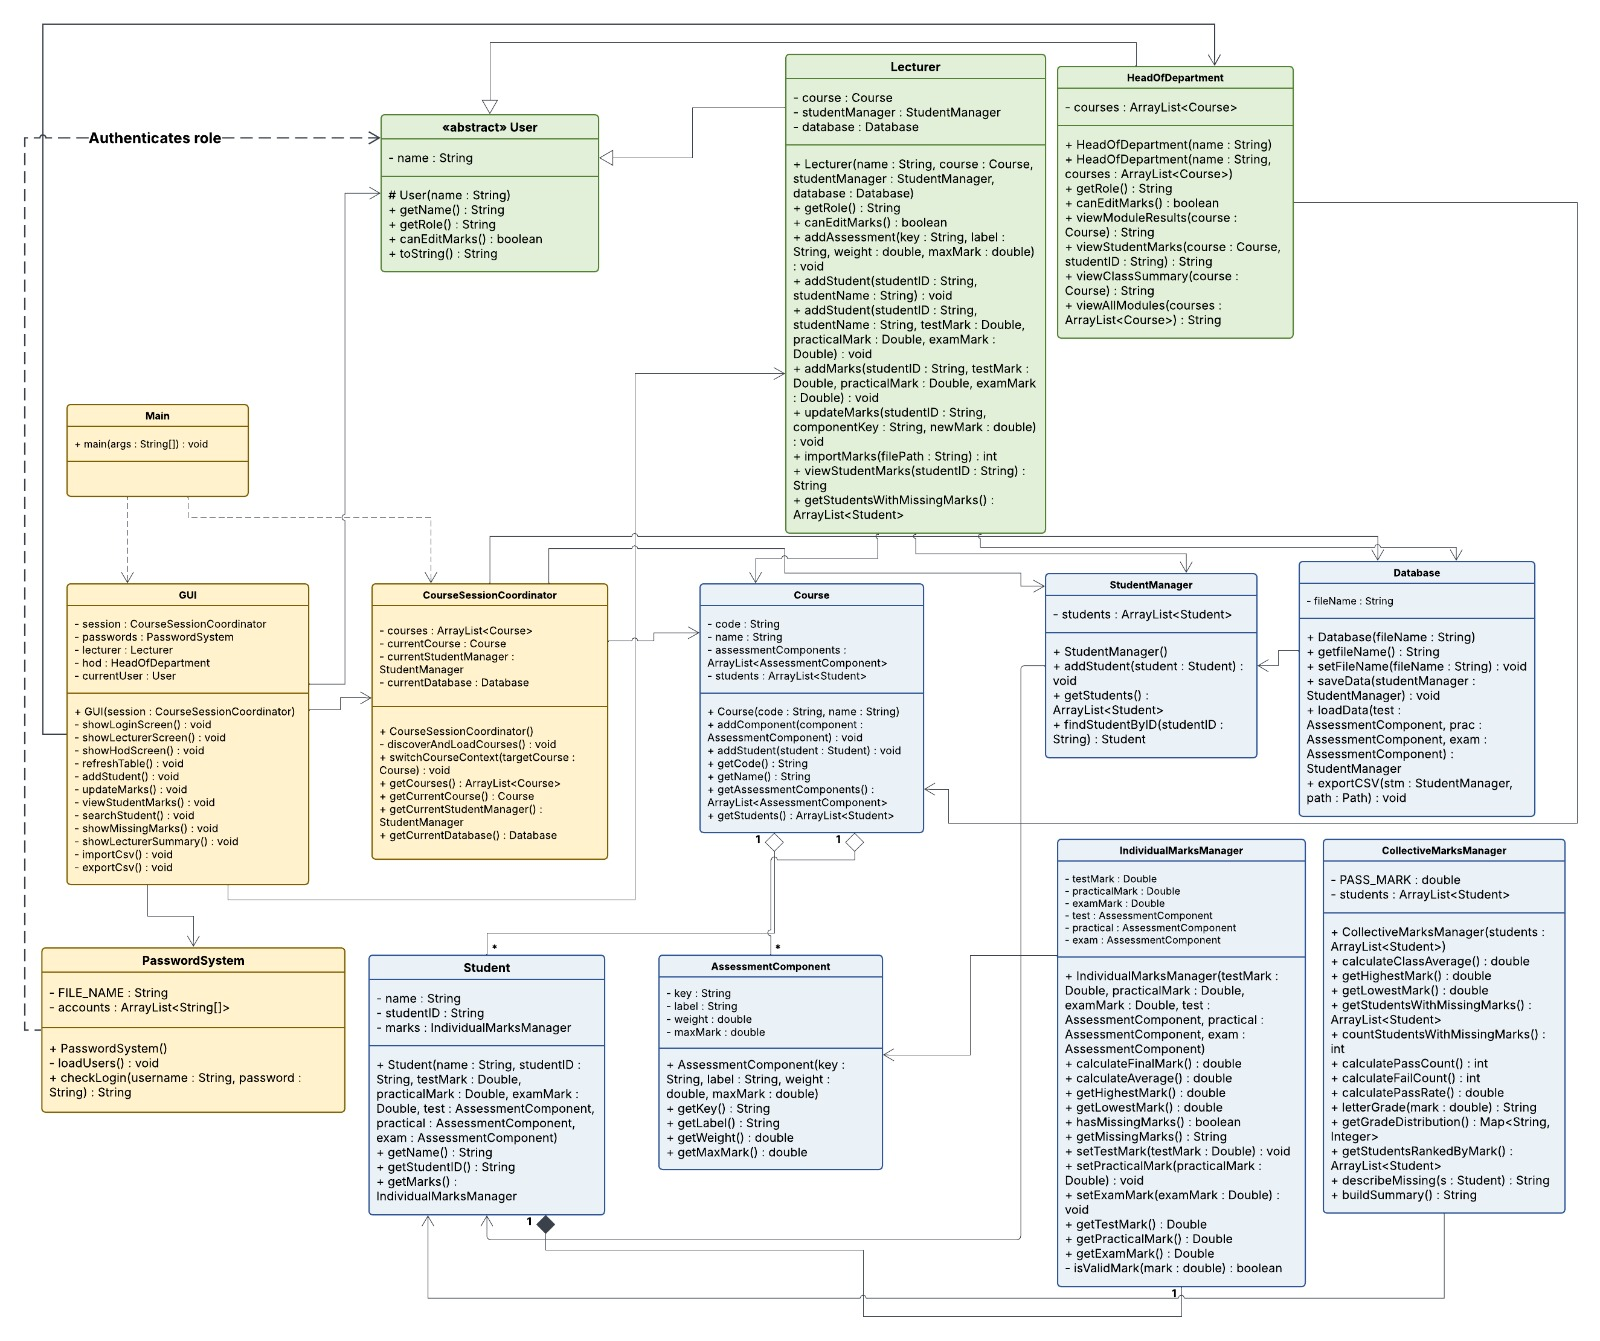
\includegraphics[width=0.9\textwidth]{Images/uml_diagram.jpeg}
    \caption{UML class diagram of the Marks Administration System.}
    \label{fig:uml}
\end{figure}

\subsection{Class responsibilities and relationships}
\begin{table}[htbp]
\centering
\footnotesize
\renewcommand{\arraystretch}{1.05}
\caption{Main classes and their responsibilities.}
\label{tab:classes}
\begin{tabularx}{\textwidth}{@{}l X@{}}
\toprule
\textbf{Class} & \textbf{Responsibility}\\
\midrule
\texttt{GUI} & Login, lecturer table and Head of Department dashboard; turns exceptions into dialogs.\\
\texttt{CourseSessionCoordinator} & Keeps the list of courses, the active course and its \texttt{StudentManager} and \texttt{Database}.\\
\texttt{User} (abstract) & Validates the name and defines the role and mark-editing permission shared by all users.\\
\texttt{Lecturer} & Adds students, captures and updates marks, imports and exports CSV, views reports.\\
\texttt{HeadOfDepartment} & Read-only inspection of course results, class summaries and student marks; manages the course list.\\
\texttt{Course} & Holds a course code and name, its assessment components and its students.\\
\texttt{AssessmentComponent} & Describes one assessment: key, label, weight and maximum mark.\\
\texttt{Student}, \texttt{StudentManager} & A student's identity and marks; the collection of students with lookup by student number.\\
\texttt{IndividualMarksManager} & Stores the three marks of one student, validates them and calculates the final mark.\\
\texttt{CollectiveMarksManager} & Class statistics, letter grades, grade distribution and rankings over complete records.\\
\texttt{Database} & Loads, saves and exports CSV files, including escaping and missing-value handling.\\
\bottomrule
\end{tabularx}
\end{table}

The relationships follow ordinary object-oriented practice. \texttt{Lecturer} and \texttt{HeadOfDepartment} \emph{inherit} from \texttt{User}, so the interface can treat both through the same type while their permissions differ. A \texttt{Course} \emph{aggregates} its assessment components and students, and each \texttt{Student} owns one \texttt{IndividualMarksManager}, which in turn \emph{refers to} three \texttt{AssessmentComponent} objects for the weights and maximum marks. \texttt{CollectiveMarksManager} only \emph{depends on} students and never modifies them. The \texttt{Database} class does not know about the interface, and the \texttt{GUI} never reads or writes files itself.
